\documentclass[tikz,border=10pt]{standalone}
\begin{document}
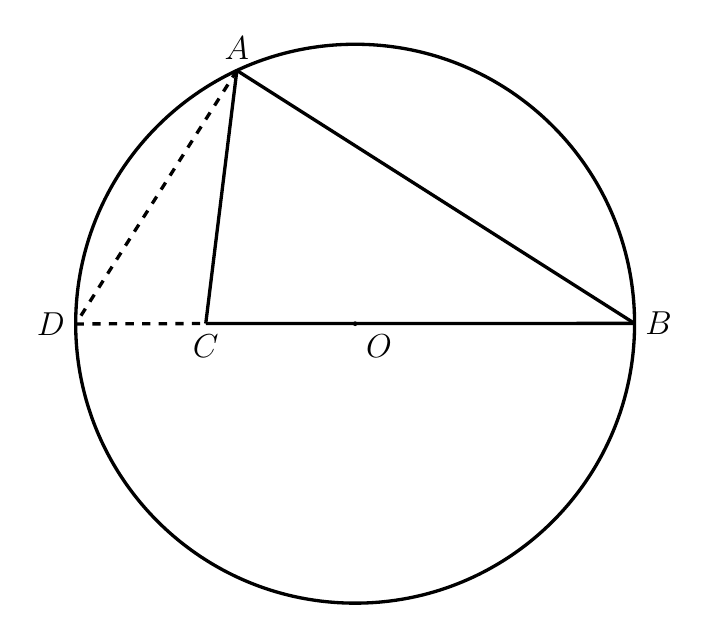
\begin{tikzpicture}[line width=1.2pt, line join=round]
\coordinate (A) at (-1.502,3.128);
\coordinate (B) at (3.548,-0.084);
\coordinate (C) at (-1.897,-0.086);
\coordinate (D) at (-3.549,-0.091);
\coordinate (O) at (0.000,-0.088);



\draw (O) circle[radius=3.549];

\draw (A) -- (B);

\draw (A) -- (C);

\draw[dashed] (A) -- (D);

\draw (C) -- (B);

\draw[dashed] (D) -- (C);

\fill (O) circle[radius=0.030];

\node[above] at (A) {\fontsize{11.5}{13.8}\selectfont $A$};
\node[right] at (B) {\fontsize{11.5}{13.8}\selectfont $B$};
\node[below] at (C) {\fontsize{11.5}{13.8}\selectfont $C$};
\node[left] at (D) {\fontsize{11.5}{13.8}\selectfont $D$};
\node[below right] at (O) {\fontsize{11.5}{13.8}\selectfont $O$};
\end{tikzpicture}
\end{document}